\colorlet{chaptergrey}{black}
%\renewcommand*\sectfont{\color{orange}}
\chapter[Discrete dynamical models of stacked dark matter haloes]{Galaxies as potential tracers: \\ Discrete dynamical models of stacked dark matter haloes in IllustrisTNG}
\label{ch:dyn_mod}
\vspace{-5.25in}
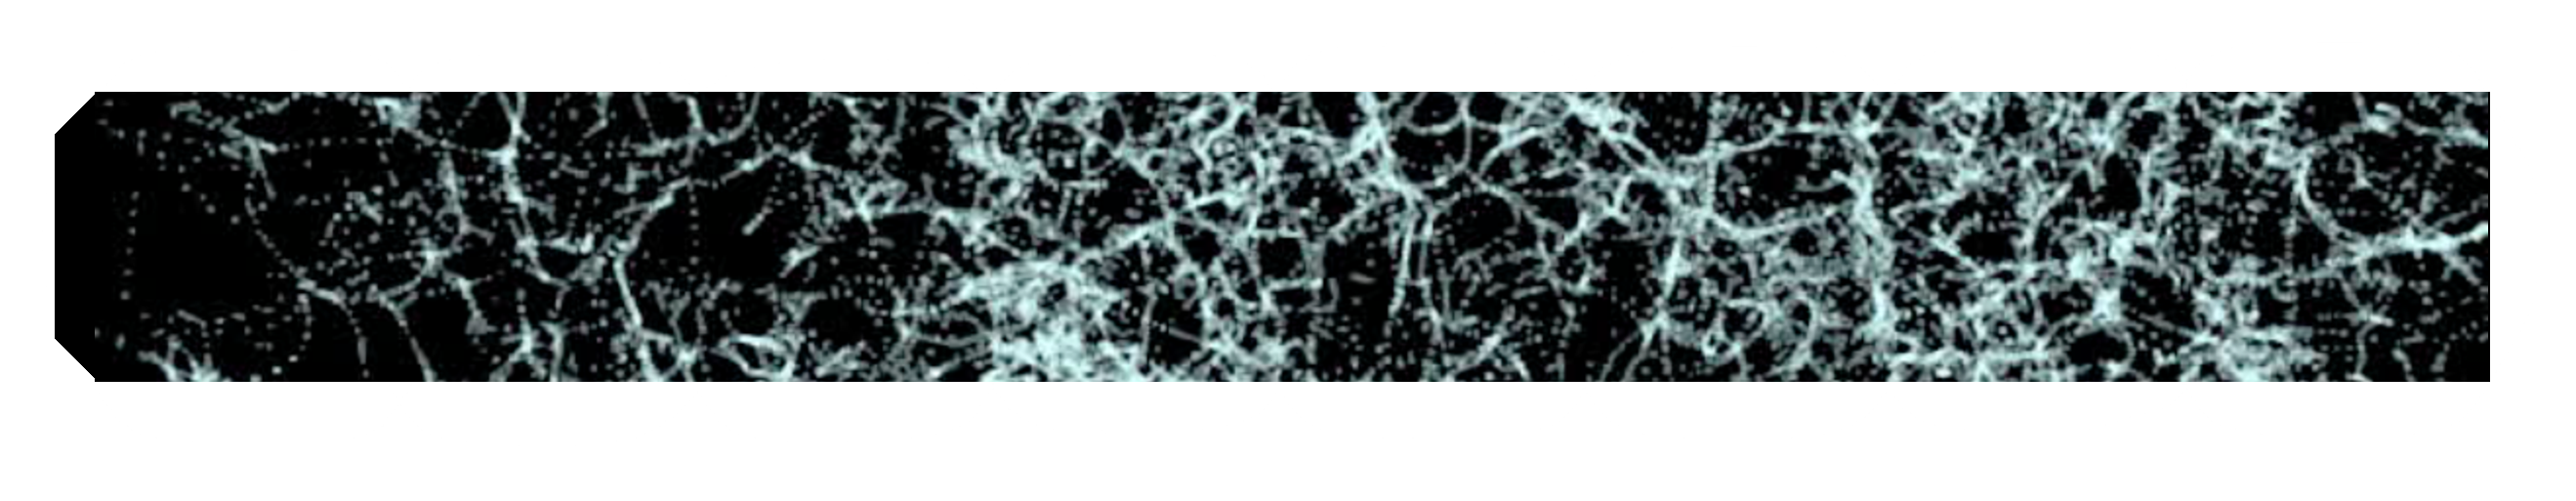
\includegraphics[height=1.39in]{thesis/latex/dyn_mod_files/tngcw_heading.pdf}
\vspace{3in}

%\epigraph{Eat slugs malfoy.}

\section{Introduction}
In the framework of the cosmic web, matter flows preferentially from under-dense to over-dense regions under the influence of the gravitational potential of the cosmic web. In Figure \ref{fig:disperse_matter_path}, we show a diagram of the flow of matter of the cosmic web, using morphological features identified by DisPerSE in IllustrisTNG300. As large-scale structure grows, material is sucked out of voids from the walls that in-case them. These walls are framed by filaments, so that matter travels along walls into the filaments, perpendicular to the filament's major axis. Once in the reference frame of the filament, material moves along its major axis, towards maxima (nodes; galaxy groups or clusters). Numerical simulations show that the natural anisotropy of the cosmic web imprints distinct signatures in the orbits of material accreting onto dark matter haloes. Haloes forming at these intersections (saddle) points should experience large degrees of anisotropy since matter is collapsing perpendicular to the filament from the walls but is moving to more dense regimes (nodes) along the direction of the filament itself \citep[e.g.][for galaxy properties in saddle environments]{kraljic2019saddle}. Outside the immediate influence of the cosmic web, lower mass dark matter halos should be able to continue to form matter more isotropically. The decrease in the tidal field strength enables the halos to continue accreting material from smaller scale filamentary structure, leading to more radial orbits.

\begin{figure*}
    \centering
	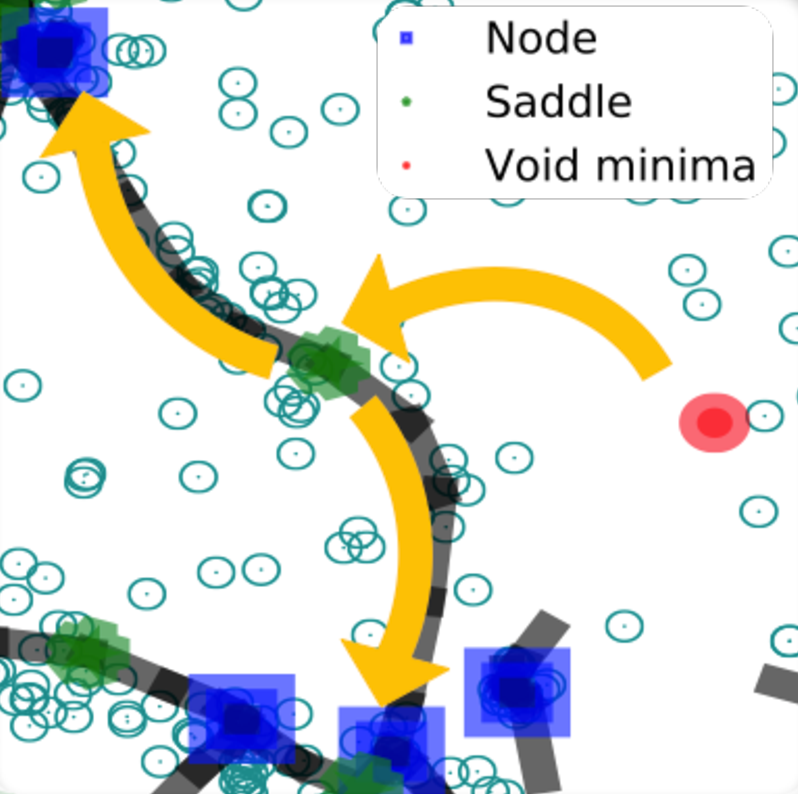
\includegraphics[width=0.5\linewidth]{thesis/latex/dyn_mod_files/disperse_matter_path.pdf}
    \caption{Representation of the flow of matter in large-scale structure. The empty green circles show the galaxy distribution in a slice of IllustrisTNG300 from which DisPerSE has been applied to. Identified nodes (blue squares), saddle points (green stars) and minima (red circles) are shown with filaments (black lines). The yellow arrows show the flow of matter to hierarchically higher mass environments. Mass is sucked out of voids which are funnelled into filaments through walls. Once within filaments, matter moves preferentially along the plane of the filament to the most over-dense regimes: nodes (galaxy groups or clusters). This flow of material inwards (perpendicular) and outwards (parallel) to a given point in the plane of the filament, creates the anisotropy we see in orbits of dark matter; \textit{especially} in saddle points.}
    \label{fig:disperse_matter_path}
\end{figure*}

In numerical simulations, the degree of perturbation from pure isotropic radial accretion is quantified by velocity anisotropy (ratio between velocity moments in tangential and radial directions). This is typically calculated by considering the total population of dark matter particles associated with the halo. On this basis, the orbits have greater tangential dispersion in haloes within environments of both higher tidal field strength and over-density \citep[e.g.][]{faltenbacher2010, shi2015}. Tidal field strength is innately related to the cosmic web, however, making a direct link to how this is modulated by filamentary structure and saddle points individually is difficult. 

Baryonic matter is also subject to the gravitational potential of the cosmic web, and, to first order, should trace the same orbits as seen in the dark matter. \citep[][]{garaldi2018} demonstrate this through considering the orbits of all satellite galaxies (albeit including those below the typical mass observable in redshift surveys) within milky way sized haloes. Satellites in those haloes embedded in (or in close vicinity to) large filamentary structure, display distinctly more anisotropic orbits, than those in isolated haloes. Being able to trace the anisotropy though satellite galaxies is promising for observations, however, recovering 3D motions for galaxies is extremely difficult.

In this chapter, we aim to trace the flow of dark matter near different morphological features of the cosmic web, through using satellite galaxies as tracers. In particular, we are interested in the impact of large scale structure on low mass dark matter haloes ($\mathrm{M_{DM} \sim 10^{12}M_{\odot}}$), whose evolution is modulated most strongly by large scale tidal fields, and hence, most likely to trace the anistropy of the cosmic web \citep[e.g.][]{tojeiro2017}. This brings an additional difficulty, as these low mass haloes will host low numbers of satellite galaxies. Using the cosmological simulation of IllustrisTNG300, we stack low mass haloes in different cosmic web environments (voids, saddle points, and filaments) to recover the difference in velocity anisotropy. To consider the dynamics within each environment we require $\sim$1000 so we stack in consistent regimes while maintaining orientation and scaling characteristic group lengths. We use this study to motivate the potential to recover the 3D motions of satellites in observations through a new application of the axisymmetric Jeans equations, and hence, the velocity anisotropy of the environment they trace. In section \S\ref{sec:dyn_mod_aniso}, we introduce the data, methodology, and results associated with using satellites galaxies as tracers in different cosmic web environments in IllustrisTNG. In section \S\ref{sec:jam}, we introduce the basics and methodology of discrete dynamical modelling, and highlight the potential for it to be used to recover 3D satellite galaxy dynamics in observations. We also present a re-derivation of the axis-symmetric jeans equations to include gravitational collapse, and removing the steady state assumption. Finally we summarise our findings and conclude in \S\ref{sec:dyn_mod_conclusions}.

\section{Anisotropy in the cosmic web} \label{sec:dyn_mod_aniso}
\subsection{Data}
\subsubsection{IllustrisTNG300}
Throughout this chapter, we base our analysis on galaxies selected from the 300Mpc box of the IllustrisTNG simulation suite. Nominally referred to as IllustrisTNG300 (TNG300), this simulation run follows the evolution of 2500$^3$ dark matter particles ($\mathrm{M_{DM} = 4 x 10^{7}h^{-1}M_{\odot}}$) and 2500$^3$ gas cells ($\mathrm{M_{gas} = 7.6 x 10^{6}h^{-1}M_{\odot}}$. The prescriptions for baryonic physics are consistent with TNG100 (see \S\ref{sec:sim_data_TNG} for further details), however TNG300 provides a far larger cosmological volume, at the cost of spatial resolution.

\subsubsection{Galaxy sample} \label{sec:gal_samp}
In parallel with TNG100, gravitationally bound structures in TNG300 are identified into haloes and subhaloes through use of a friends-of-friends algorithm \citep{davis85} and the subfind algorithm \citep{springel01} respectively (see \S\ref{sec:sim_data_TNG}). In this work, we select a galaxy sample in TNG300 by considering all $z=0$ (snapshot 99) subhaloes which contain a minimum stellar mass of $\mathrm{M_{\ast} = 10^{8} M_{\odot}}$ within a 3D aperture of 30 comoving kpc from the subhalo centre \citep[as defined in;][]{pillepich18b}. This corresponds to 564,930 unique galaxies which we use for both reconstruction of the cosmic web, and for the satellite tracers in the velocity anisotropy calculations.

In the context of halo assembly, we are particularly interested in isolating the impact of the cosmic web on low mass dark matter haloes. To this effect, we select all galaxies (from our sample above) that reside in a FoF halo of mass $\mathrm{10^{11.5} M_{\odot} < M_{h} < 10^{12.5} M_{\odot}}$, which we use to stack in each cosmological environment as described in \S\ref{sec:stacking}. 

\subsubsection{Cosmological environment}
To identify morphological features of the cosmic web, we make use of DisPerSE (see \S\ref{sec:cosmic_web_intro} for more information). We apply DisPerSE directly to the spatial distribution of our selected galaxy sample in the periodic cube of TNG300. In Figure \ref{fig:disperse_TNG300}, we show the spatial distribution of galaxies for a 10Mpc slice through TNG300, along with the identified filamentary network from DisPerSE.

\begin{figure*}
	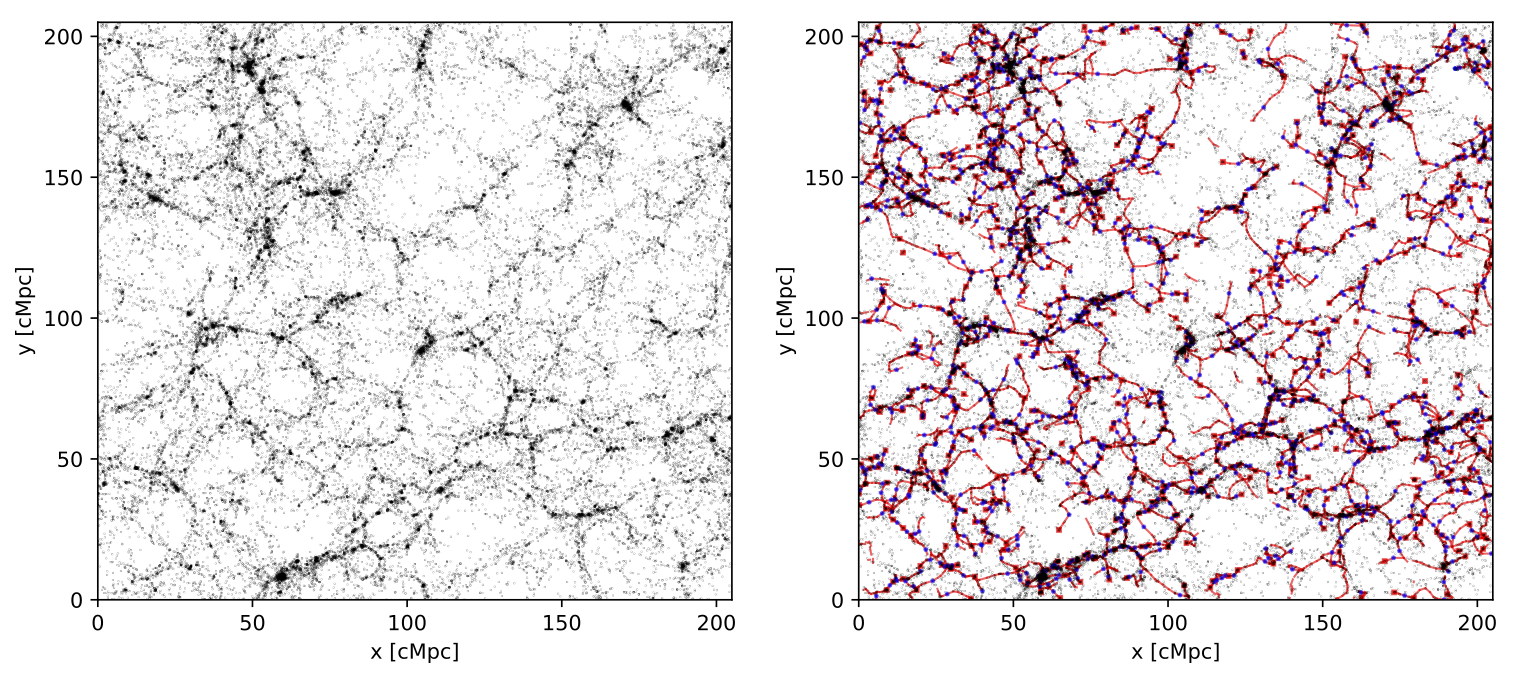
\includegraphics[width=\linewidth]{dyn_mod_files/TNG300-1-SM10-8-slice-galaxy-density-skeleton-comparison.png}
    \caption{Illustration of the filamentary network identified from galaxy positions within a 10 Mpc slice in TNG. The left panel shows the distribution of galaxy ($\mathrm{M_{\ast} > 10^{8}M_{\odot}}$) positions within the slice. The right panel shows the same but with filamentary structure overlaid (red lines). Critical points are also shown such as nodes (red squares) and saddle points (blue stars) highlighting the ensemble which the skeleton connects.}
    \label{fig:disperse_TNG300}
\end{figure*}

Having constructed a skeleton of the cosmic web, we now look to classify the selected haloes into distinct cosmological environments. In similarity with \S\ref{sec:cosmic_web_distances}, for each FoF halo (computed from the centre point), the distance to the nearest node ($\mathrm{D_{node}}$), filament segment ($\mathrm{D_{skel}}$) and saddle point ($\mathrm{D_{2-saddle}}$) is found. 

\subsection{Stacking of cosmic web environments} \label{sec:stacking}
In order to trace the differences in orbits for different cosmic web environments with satellite galaxies, we need enough tracers to first compute the anisotropy directly, and further, enough to test the feasibility of computing the anisotropy in observations. Since our focus is the impact on low mass haloes, we only have a handful (at best) of satellite galaxies to use as tracers. To proceed, we therefore must stack similar haloes in the same topological environment. 

For each environment (node, filament, saddle point) we select all galaxies in FoF haloes with $\mathrm{10^{11.5} M_{\odot} < M_{h} < 10^{12.5} M_{\odot}}$. To ensure we are only selecting FoF haloes that are only subject to a certain morphological feature and hence remove effects due to the proximity of other environments, we take all those within the following conservative selections as shown in Table \ref{tab:stacking}. 

\begin{table}
\centering
\begin{tabular}{|l|c|c|c|}
\hline
& Filament & 2-saddle & Void \\ \hline
$D_{node}$ & > 2 Mpc & > 2 Mpc & > 5 Mpc \\
$D_{skel}$ & < 0.5 Mpc  & - - & > 5 Mpc \\
$D_{2-saddle}$ & > 1 Mpc & < 0.75 Mpc & > 5 Mpc \\
Number of galaxies: & 8071 & 941 & 2246 \\
\hline
\end{tabular}
\caption{Selection criteria for stacks in three different environments; filaments, 2-saddle points and voids. Each row shows the distance cut used to select an environment apart from the final row which shows the total number of galaxies selected.}
\label{tab:stacking}
\end{table}

In order to stack dark matter potentials and their tracers for the purpose of dynamical modelling, we must be careful about orientation, scaling and effects resulting due to the proximity of other environments. To construct a reliable dynamical model, all tracers should reside in gravitational potentials that are consistent in overall mass and scale. For every FoF halo that contains a galaxy to be stacked we take the density profile and scale it according to the characteristic group scale as defined by $R_{200}$ (comoving radius of a sphere centered on the FoF halo whose mean density is 200 times the critical density of the Universe). The magnitude of the density profile is scaled according to the total mass contained in the FoF halo and then combined so that each stacked density profile contributes equally to the final profile. The stacked FoF halo density profile is finally scaled so that its total mass is equal to the median for the stacked population. We then convert the final density profile to the gravitational potential as described in \ref{sec:grav_pot}.

Each tracer position and velocity is also scaled by the characteristic group scale of its host FoF halo, $\mathrm{R_{200}}$. \red{Should velocity be scaled according to mass or is this accounted for by the scale?}. 

A natural assumption of our Jeans formalism is symmetry around the principal axis of rotation, so it is important to retain directionality while stacking tracers and potentials. In the instance of 2-saddle points and filaments, we use the direction of the nearest filament segment (from 2-saddle to node) to stack along. For those stacked in the void environments we use the direction of the angular momentum vector for the central subhalo. \red{Do this from stellar only?, do this for whole FoF halo? - check correlation?}

\subsection{Velocity anisotropy}
On a particle level, the orbits within FoF haloes have been shown to be dependent on large scale environment. \citet{faltenbacher2010} used an implementation of the Tree-PM N-body code GADGET2 on-top of the Millenium simulation. They examine the correlation between clustering and halo properties such as shape, concentration, spin, shape of the velocity ellipsoid and velocity anisotropy. The velocity anisotropy parameter is defined as
\begin{equation} \label{eq:vel_ani_sigma}
\mathrm{\beta_{\sigma}(r) = 1 - \frac{\sigma_t^2(r)}{\sigma_r^2(r)} }
\end{equation}
where $\sigma_r^2(r)$ and $\sigma_t^2(r)$ denote the radial and tangential velocity dispersions. Note that this equation can also be presented as an average for a halo. 

They determine that $\beta_{\sigma}$ is most tightly correlated with the clustering strength, with halos of low velocity anisotropy being more highly clustered and the opposite holding true for haloes with strongly radially biased velocities. 

A possible explanation for more highly clustered haloes exhibiting a relatively larger tangential velocity dispersion is that the impact parameters of the merging sub-haloes are larger due to far more gravitational interactions a short time before accretion. This would lead to a greater dispersion of tangential velocities corresponding to a lower velocity anisotropy. On the other hand, in less clustered regions the gravitational field is dominated by the halo itself naturally leading to more radial in-fall. 

Further, velocity anisotropy has also been decomposed as a function of tidal environment. \cite{shi2015} investigate how halo dynamical properties are related to their formation histories and hence the tidal environment in which they reside. They demonstrate a clear correlation between $\beta_{\sigma}$ and the first eigenvalue of the tidal tensor (i.e. tidal field strength) for both low mass and high mass haloes. As tidal field strength increases, $\beta_{\sigma}$ decreases, showing that again there is a greater dispersion in tangential orbits. 

In the right panel of Figure \ref{fig:beta_stack}, we show $\beta_{\sigma}$ calculated directly from the satellite tracers in our void (red, dotted), filament (black, dot-dashed) and 2-saddle (green, solid) stacks. Within 0.1 Mpc of the halo centre, $\beta_{\sigma}$ is roughly consistent between environments. Above 0.1 Mpc, however, there is a clear difference between the three environments with 2-saddles exhibiting a relatively larger tangential velocity dispersion and voids displaying more isotropic orbits. The gray box inlaid in the panel shows $\overline{\beta_{\sigma}}$ calculated from all satellite tracers. The clear difference between voids, filaments and 2-saddles dictates that trends previously shown on a particle level can be recovered from satellites as tracers. 

\begin{figure*}
	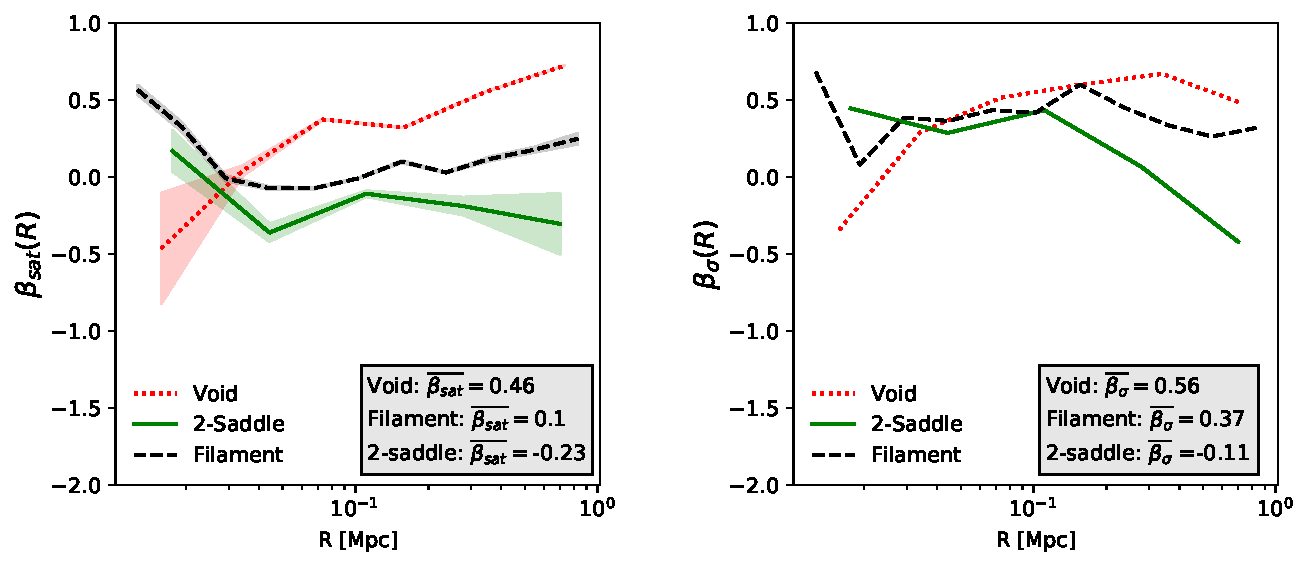
\includegraphics[width=\linewidth]{thesis/latex/dyn_mod_files/disperse_beta_paper.pdf}
    \caption{Velocity anisotropy profiles found from satellite galaxies in the void (red, dotted), filament (black, dot-dashed) and 2-saddle (green, solid) stacks. The left (right) panel corresponds to $\beta_{sat}$ ($\beta_{\sigma}$) with the shaded regions showing error on the mean. The average value for all satellites in each stack is shown in the grey box. For both $\beta_{sat}$ and $\beta_{\sigma}$, there is a clear distinction in orbital anisotropy between environments which increases with radii.}
    \label{fig:beta_stack}
\end{figure*}

The orbits of satellite galaxies in the context of the cosmic web has been previously considered in a set of zoom N-body and hydrodynamical simulations \citep{ZOMGiii}. They define the satellite anisotropy parameter as
\begin{equation}
\beta_{sat}(r) = 1 - \frac{v_{t}^2(r)}{v_{r}^{2}(r)} 
\end{equation}
where $v_{t}(r)$ and $v_{r}(r)$ denote the radial and tangential velocities. They follow seven galaxy sized haloes ($M_{h} \sim 10^{11} M_{\odot}$) which are classified as `stalled' or accreting corresponding to the time at which their final mass becomes stable. The accreting haloes correspond with \green{voids?} nodes of the cosmic web and are fed isotropically by radial infall of matter along filaments. Conversely `stalled' haloes are embedded in prominent filaments of the large-scale structure. They find that the satellite anisotropy parameter at $z = 0$ is positive for accreting haloes and negative for stalled haloes showing that orbits become more tangentially biased (both in magnitude and dispersion) when low mass haloes are closer to large filamentary structure. 

In the left panel of Figure \ref{fig:beta_stack}, we show $\beta_{sat}$ again calculated directly from the satellite tracers in our void (red, dotted), filament (black, dot-dashed) and 2-saddle (green, solid) stacks. We again see a clear distinction between environments in the anisotropy with 2-saddles exhibiting orbits with stronger tangential velocity components at larger radii. The gray box inlaid shows $\overline{\beta_{sat}}$ found from all satellites within the stacks. In-keeping with \citet{ZOMGiii}, we find that the satellite anisotropy becomes more tangentially biased as we more closer to large filamentary structure.

It should be noted that while it is important to retain directionality in stacking for the purpose of dynamical modelling, it has no impact on the direct measures of $\beta_{\sigma}$ and $\beta_{sat}$.

\section{Potential applications of discrete dynamical models} \label{sec:jam}


\subsection{Generalised Jeans equations in cylindrical coordinates}
In standard cylindrical coordinates (R,z,$\phi$) under the assumption of axial symmetry (so that; $\partial \Phi / \partial \phi = \partial f / \partial \phi = 0$) we find the collisionless Boltzmann equation to be (cf. BT equation [4-17]): 
\begin{equation} \label{eq:CBE}
\frac{\partial f}{\partial t} + v_R \frac{\partial f}{\partial R} + v_z \frac{\partial f}{\partial z} + \left[\frac{v_{\phi}^2}{R} - \frac{\partial \Phi}{\partial R}\right] \frac{\partial f}{\partial v_R} - \frac{v_R v_{\phi}}{R} \frac{\partial f}{\partial v_{\phi}} - \frac{\partial \Phi}{\partial z} \frac{\partial f}{\partial V_z} = 0.
\end{equation}

Without making the usual assumptions of steady state, we multiply equation \ref{eq:CBE} by $v_{R}$ and $v_z$ respectively and integrate over all velocities to obtain (Jeans 1922, BT equation [4-29a,c])
\begin{align} \label{eq:j_vr}
\frac{\partial (\nu \overline{v_R})}{\partial t} + \frac{\partial (\nu \overline{v_R^2})}{\partial R} + \frac{\partial (\nu \overline{v_R v_z})}{\partial z} + \nu \left[ \frac{\overline{v_R^2} - \overline{v_{\phi}^2}}{R} + \frac{\partial \Phi}{\partial R}\right] &= 0\\ \label{eq:j_vz}
\frac{\partial (\nu \overline{v_z})}{\partial t} + \frac{\partial (\nu \overline{v_R v_z})}{\partial R} + \frac{\partial (\nu \overline{v_z^2})}{\partial z} + \nu \frac{\overline{v_R v_z}}{R} + \nu \frac{\partial \Phi}{\partial z}&= 0.
\end{align}
where we use the following notation
\begin{align}
\nu &\equiv \int f d^3 v \\
\nu \overline{v_k v_j} &\equiv \int v_k v_j f d^3 v .
\end{align}
Similarly we can derive the continuity equation in cylindrical coordinates by integrating \ref{eq:CBE} over all velocities (cf. BT [4-28] 
\begin{equation} \label{eq:contin}
\frac{\partial \nu}{\partial t} + \frac{1}{R}\frac{\partial (R \nu \overline{v_R})}{\partial R} + \frac{\partial (\nu \overline{v_z})}{\partial z} = 0.
\end{equation}
We wish to now go beyond the assumption of steady state and allow net radial motion due to the infall and collapse of dark matter haloes (i.e. $\overline{v_r} \neq 0$, $\overline{v_z} \neq 0$). The second order velocity moments therefore can be written as:
\begin{align} \label{eq:vr}
\overline{v_R^2} &= \sigma_R^2 + \overline{v_R}^2 \\ \label{eq:vz}
\overline{v_z^2} &= \sigma_z^2 + \overline{v_z}^2
\end{align}
We can now make use of the continuity equation \ref{eq:contin} and rewrite the first term in \ref{eq:j_vr};
\begin{align}
\frac{\partial ( \nu \overline{v_R})}{\partial t} &= \nu \frac{\partial \overline{v_R}}{\partial t} + \overline{v_R} \frac{\partial \nu}{\partial t} \\
&= \nu \frac{\partial \overline{v_R}}{\partial t} - \overline{v_R}\frac{\partial (\nu \overline{v_z})}{\partial z} - \frac{\nu}{R}\overline{v_R}^2 - \overline{v_R} \frac{\partial (\nu \overline{v_R})}{\partial R}.
\end{align}
We can also rewrite the second term in equation \ref{eq:j_vr} through use of equation \ref{eq:vr} and the product rule; 
\begin{align}
\frac{\partial ( \nu \overline{v_R^2})}{\partial R} &= \frac{\partial (\nu \sigma^2_R)}{\partial R} + \frac{\partial ( \nu \overline{v_R}^2)}{\partial R} \\
&= \frac{\partial (\nu \sigma^2_R)}{\partial R} +  \overline{v_R}\frac{\partial (\nu \overline{v_R})}{\partial R} + \nu \overline{v_R} \frac{\partial \overline{v_R}}{\partial R}.
\end{align}
Re-introducing these terms and using a similar method for the $v_z$ moment, the Jeans equations (\ref{eq:j_vr},\ref{eq:j_vz}) can be rewritten as
\begin{multline}
\nu \left[\overline{v_R}\frac{\partial \overline{v_R}}{\partial R} + \frac{\partial \overline{v_R}}{\partial t} \right] - \overline{v_R} \frac{\partial (\nu \overline{v_z})}{\partial z} + \frac{\partial (\nu \sigma_R^2)}{\partial R} + \frac{\partial (\nu \overline{v_R v_z})}{\partial z} + \nu \left[ \frac{\sigma_R^2 - \overline{v_{\phi}^2}}{R} + \frac{\partial \Phi}{\partial R}\right] = 0
\end{multline}
\begin{multline}
\nu \left[\overline{v_z}\frac{\partial \overline{v_z}}{\partial z} + \frac{\partial \overline{v_z}}{\partial t} \right] - \overline{v_z} \frac{\partial (\nu \overline{v_R})}{\partial R} + \frac{\partial (\nu \sigma_z^2)}{\partial z} + \frac{\nu \sigma_{Rz}^2}{R} + \nu \frac{\partial \Phi}{\partial z} = 0 
\end{multline}
where we have used that $\overline{v_z v_R} = \sigma_{Rz}^2 + \overline{v_R} \ \overline{v_z}$. These reduce to the usual form of the Jeans equations under the steady state assumption but due to this inclusion of non-equilibrium, we find three additional terms in both relating to the mean radial motion of galaxies in both the $z$ and $R$ directions.

\section{Summary and Conclusions} \label{sec:dyn_mod_conclusions}